\section{$3$-valent {\sc Eberhard}-like theorems with triangles}\label{sec:3:3}

In this section we want to prove $3$-valent {\sc Eberhard}-like theorems with triangles, i.e. for $q = [q_3 \times 3, q_l \times l]$, $w = [w_3 \times 3]$, $l > 6$, $\gcd(q_3, q_l) = 1$. As it turns out in \autoref{sec:negative:results}, this is only possible for all admissible pairs of sequences on all closed orientable $2$-manifolds in three cases: $q = [3, 3 \times 7]$, $q = [2 \times 3, 3 \times 8]$ and $q = [4 \times 3, 3 \times 10]$. We tackle each case separately in the following three theorems.

\begin{theorem}
  Let $p$ and $v$ be a pair of admissible sequences for a orientable closed $2$-manifold $S$. Then $(p, v)$ is $[3, 3 \times 7]$-$[3]$-realizable.
  \begin{proof}
    An expansion $3$-patch with outer tuple $o = (2, 1, 2, 2, 2, 1, 1, 1, 2, 1)$ and a corresponding $o$-$6$-gonal $3$-patch, both consisting only of triangles and heptagons is shown in \autoref{fig:expansion:patch:3:7}. Since the expansion patch is already polyhedral, we can apply \autoref{thm:main:const}.
    \begin{tikzfigure}{\label{fig:expansion:patch:3:7}}{\todo{caption, rework expansion patch}}
      \matrix (m) [column sep=1cm] {

        \begin{scope}[yscale=0.866, scale=0.8]

          \coordinate (p0)  at  (0,0);
          \coordinate (p1)  at  (0.5,1);
          \coordinate (p2)  at  (1.5,5);
          \coordinate (p3)  at  (0.500,10.600);
          \coordinate (p4)  at  (-0.5,11);
          \coordinate (p5)  at  (-1.5,11.666);
          \coordinate (p6)  at  (-2.5,13.666);
          \coordinate (p7)  at  (-3.5,11.666);
          \coordinate (p8)  at  (-4.5,11);
          \coordinate (p9)  at  (-4.5,9.666);
          \coordinate (p10) at  (-3.5,7.666);
          \coordinate (p11) at  (-5.5,7.666);
          \coordinate (p12) at  (-6.5,7);
          \coordinate (p13) at  (-7.3,6.2);
          \coordinate (p14) at  (-7.2,4.8);
          \coordinate (p15) at  (-2.5,3);
          \coordinate (p16) at  (-2.5,7);

          \node[anchor= 90] at (p0) {$i_{0}$};
          \node[anchor=180] at (p1) {$i_0'$};
          \node[anchor=180] at (p2) {$i_1'$};
          \node[anchor=180] at (p3) {$i_2'=o_{11}$};
          \node[anchor=270] at (p4) {$o_{10}$};
          \node[anchor=200] at (p5) {$o_{9}$};
          \node[anchor=270] at (p6) {$o_{8}$};
          \node[anchor=340] at (p7) {$o_{7}$};
          \node[anchor=  0] at (p8) {$o_{6}$};
          \node[anchor=330] at (p9) {$o_{5}$};
          \node[anchor=330] at (p10){$o_{4}$};
          \node[anchor=270] at (p11){$o_{3}$};   
          \node[anchor=340] at (p12){$o_{2}$};
          \node[anchor=  0] at (p13){$o_{1}$}; 
          \node[anchor= 90] at (p14){$i_2=o_0$};
          \node[anchor= 90] at (p15){$i_1$};
          
          \draw[very thick](p0)-- (p1)-- (p2)-- (p3)-- (p4)-- (p5)-- (p6)-- (p7)-- (p8)-- (p9)-- (p10)-- (p11)-- (p12)-- (p13)-- (p14)--(p15)-- (p0) ;

          \draw (p15)--(p16)--(p4);
          \draw (p16)--(p10);
          \draw (p7) -- (p5);
          
        \end{scope} 

        &
        % \documentclass[a4paper]{article}
\usepackage[left=0.5cm, right=0.5cm, top=1cm, bottom=1cm]{geometry}
\usepackage{tikz}
\begin{document}
\begin{figure}[h!]
\centering
\begin{tikzpicture}[scale = 10, auto]
\coordinate (x0) at (-0.011576, -0.166942);
\coordinate (x1) at (0.321662, -0.461316);
\coordinate (x2) at (0.654861, -0.755750);
\coordinate (x3) at (0.959493, -0.281733);
\coordinate (x4) at (-1.000000, 0.000000);
\coordinate (x5) at (-0.841254, -0.540641);
\coordinate (x6) at (-0.415415, -0.909632);
\coordinate (x7) at (0.142315, -0.989821);
\coordinate (x8) at (0.959493, 0.281733);
\coordinate (x9) at (0.142315, 0.989821);
\coordinate (x10) at (-0.415415, 0.909632);
\coordinate (x11) at (-0.841254, 0.540641);
\coordinate (x12) at (0.654861, 0.755750);
\draw (-0.011576, -0.166942) -- (0.321662, -0.461316);
\draw (0.321662, -0.461316) -- (0.654861, -0.755750);
\draw (0.654861, -0.755750) -- (0.959493, -0.281733);
\draw (0.959493, -0.281733) -- (-0.011576, -0.166942);
\draw (-0.011576, -0.166942) -- (-1.000000, 0.000000);
\draw (-1.000000, 0.000000) -- (-0.841254, -0.540641);
\draw (-0.841254, -0.540641) -- (-0.415415, -0.909632);
\draw (-0.415415, -0.909632) -- (0.142315, -0.989821);
\draw (0.142315, -0.989821) -- (0.654861, -0.755750);
\draw (0.959493, -0.281733) -- (0.959493, 0.281733);
\draw (0.959493, 0.281733) -- (0.142315, 0.989821);
\draw (0.142315, 0.989821) -- (-0.415415, 0.909632);
\draw (-0.415415, 0.909632) -- (-0.841254, 0.540641);
\draw (-0.841254, 0.540641) -- (-1.000000, 0.000000);
\draw (0.959493, 0.281733) -- (0.654861, 0.755750);
\draw (0.654861, 0.755750) -- (0.142315, 0.989821);
\node at (-0.000000, -0.000000) {0};
\node at (0.481110, -0.416435) {1};
\node at (-0.164201, -0.546300) {2};
\node at (-0.029563, 0.324736) {3};
\node at (0.585556, 0.675768) {4};
\end{tikzpicture}
\caption{Graph}

\end{figure}
\end{document}

        \begin{scope}[scale=0.5]
          \begin{scope}[yscale=0.866]

            \coordinate (p0)  at  (0,0) ;
            \coordinate (p1)  at  (0.5,1)  ;
            \coordinate (p2)  at  (1.5,5)  ;
            \coordinate (p3)  at  (0.500,10.600);
            \coordinate (p4)  at  (-0.5,11)  ;
            \coordinate (p5)  at  (-1.5,11.666)  ;
            \coordinate (p6)  at  (-2.5,13.666)  ;
            \coordinate (p7)  at  (-3.5,11.666)  ;
            \coordinate (p8)  at  (-4.5,11);
            \coordinate (p9)  at  (-4.5,9.666) ;
            \coordinate (p10) at  (-3.5,7.666);
            \coordinate (p11) at  (-5.5,7.666)  ;     
            \coordinate (p12) at  (-6.5,7) ;        
            \coordinate (p13) at  (-7.3,6.2);    
            \coordinate (p14) at  (-7.2,4.8)  ;
            \coordinate (p15) at  (-2.5,3);
            \coordinate (p16) at  (-2.5,7)  ;
            
            \draw[very thick](p0)-- (p1)-- (p2)-- (p3)-- (p4)-- (p5)-- (p6)-- (p7)-- (p8)-- (p9)-- (p10)-- (p11)-- (p12)-- (p13)-- (p14)--(p15)-- (p0) ;

            \draw (p15)--(p16)--(p4);
            \draw (p16)-- (p10);
            \draw (p7) -- (p5);
          \end{scope}        
          
          \begin{scope}[rotate=-60,xshift=-0.5cm,yshift=0.866cm,yscale=0.866]

            \coordinate (p0)  at  (0,0) ;
            \coordinate (p1)  at  (0.5,1)  ;
            \coordinate (p2)  at  (1.5,5)  ;
            \coordinate (p3)  at  (0.500,10.600);         
            \coordinate (p4)  at  (-0.5,11)  ;
            \coordinate (p5)  at  (-1.5,11.666)  ;
            \coordinate (p6)  at  (-2.5,13.666)  ;
            \coordinate (p7)  at  (-3.5,11.666)  ;
            \coordinate (p8)  at  (-4.5,11);
            \coordinate (p9)  at  (-4.5,9.666) ;
            \coordinate (p10) at  (-3.5,7.666);
            \coordinate (p11) at  (-5.5,7.666)  ;     
            \coordinate (p12) at  (-6.5,7) ;        
            \coordinate (p13) at  (-7.3,6.2);    
            \coordinate (p14) at  (-7.2,4.8)  ;
            \coordinate (p15) at  (-2.5,3);
            \coordinate (p16) at  (-2.5,7)  ;
            
            \draw[very thick](p0)-- (p1)-- (p2)-- (p3)-- (p4)-- (p5)-- (p6)-- (p7)-- (p8)-- (p9)-- (p10)-- (p11)-- (p12)-- (p13)-- (p14)--(p15)-- (p0) ;

            \draw (p15)--(p16)--(p4);
            \draw (p16)-- (p10);
            \draw (p7) -- (p5);
          \end{scope}

          \begin{scope}[xshift=2cm,yshift=19.0666cm, rotate=-180,yscale=0.866]

            \coordinate (p0)  at  (0,0) ;
            \coordinate (p1)  at  (0.5,1)  ;
            \coordinate (p2)  at  (1.5,5)  ;
            \coordinate (p3)  at  (0.500,10.600);         
            \coordinate (p4)  at  (-0.5,11)  ;
            \coordinate (p5)  at  (-1.5,11.666)  ;
            \coordinate (p6)  at  (-2.5,13.666)  ;
            \coordinate (p7)  at  (-3.5,11.666)  ;
            \coordinate (p8)  at  (-4.5,11);
            \coordinate (p9)  at  (-4.5,9.666) ;
            \coordinate (p10) at  (-3.5,7.666);
            \coordinate (p11) at  (-5.5,7.666)  ;     
            \coordinate (p12) at  (-6.5,7) ;        
            \coordinate (p13) at  (-7.3,6.2);    
            \coordinate (p14) at  (-7.2,4.8)  ;
            \coordinate (p15) at  (-2.5,3);
            \coordinate (p16) at  (-2.5,7)  ;
            
            \draw[very thick](p0)-- (p1)-- (p2)-- (p3)-- (p4)-- (p5)-- (p6)-- (p7)-- (p8)-- (p9)-- (p10)-- (p11)-- (p12)-- (p13)-- (p14)--(p15)-- (p0) ;

            \draw (p15)--(p16)--(p4);
            \draw (p16)-- (p10);
            \draw (p7) -- (p5);
          \end{scope}
          \begin{scope}[xshift=1.5cm,yshift=18.2cm, rotate=-240,yscale=0.866]

            \coordinate (p0)  at  (0,0) ;
            \coordinate (p1)  at  (0.5,1)  ;
            \coordinate (p2)  at  (1.5,5)  ;
            \coordinate (p3)  at  (0.500,10.600);         
            \coordinate (p4)  at  (-0.5,11)  ;
            \coordinate (p5)  at  (-1.5,11.666)  ;
            \coordinate (p6)  at  (-2.5,13.666)  ;
            \coordinate (p7)  at  (-3.5,11.666)  ;
            \coordinate (p8)  at  (-4.5,11);
            \coordinate (p9)  at  (-4.5,9.666) ;
            \coordinate (p10) at  (-3.5,7.666);
            \coordinate (p11) at  (-5.5,7.666)  ;     
            \coordinate (p12) at  (-6.5,7) ;        
            \coordinate (p13) at  (-7.3,6.2);    
            \coordinate (p14) at  (-7.2,4.8)  ;
            \coordinate (p15) at  (-2.5,3);
            \coordinate (p16) at  (-2.5,7)  ;
            
            \draw[very thick](p0)-- (p1)-- (p2)-- (p3)-- (p4)-- (p5)-- (p6)-- (p7)-- (p8)-- (p9)-- (p10)-- (p11)-- (p12)-- (p13)-- (p14)--(p15)-- (p0) ;

            \draw (p15)--(p16)--(p4);
            \draw (p16)-- (p10);
            \draw (p7) -- (p5);
          \end{scope} 
        \end{scope}
        \\
      };
    \end{tikzfigure}
    % \begin{tikzfigure}{\label{fig:expansion:patch:poly:3:7}}{\todo{caption}}
    %   \begin{scope}[scale=3]
    %     \documentclass[a4paper]{article}
\usepackage[left=0.5cm, right=0.5cm, top=1cm, bottom=1cm]{geometry}
\usepackage{tikz}
\begin{document}
\begin{figure}[h!]
\centering
\begin{tikzpicture}[scale = 10, auto]
\coordinate (x0) at (-0.766044, -0.642788);
\coordinate (x1) at (-0.530999, -0.345988);
\coordinate (x2) at (-0.296173, -0.049085);
\coordinate (x3) at (-1.000000, 0.000000);
\coordinate (x4) at (-0.173648, -0.984808);
\coordinate (x5) at (0.500000, -0.866025);
\coordinate (x6) at (0.939693, -0.342020);
\coordinate (x7) at (0.430143, -0.014828);
\coordinate (x8) at (0.939693, 0.342020);
\coordinate (x9) at (0.500000, 0.866025);
\coordinate (x10) at (-0.173648, 0.984808);
\coordinate (x11) at (-0.766044, 0.642788);
\draw (-0.766044, -0.642788) -- (-0.530999, -0.345988);
\draw (-0.530999, -0.345988) -- (-0.296173, -0.049085);
\draw (-0.296173, -0.049085) -- (-1.000000, 0.000000);
\draw (-1.000000, 0.000000) -- (-0.766044, -0.642788);
\draw (-0.766044, -0.642788) -- (-0.173648, -0.984808);
\draw (-0.173648, -0.984808) -- (0.500000, -0.866025);
\draw (0.500000, -0.866025) -- (0.939693, -0.342020);
\draw (0.939693, -0.342020) -- (0.430143, -0.014828);
\draw (0.430143, -0.014828) -- (-0.296173, -0.049085);
\draw (0.939693, -0.342020) -- (0.939693, 0.342020);
\draw (0.939693, 0.342020) -- (0.430143, -0.014828);
\draw (0.939693, 0.342020) -- (0.500000, 0.866025);
\draw (0.500000, 0.866025) -- (-0.173648, 0.984808);
\draw (-0.173648, 0.984808) -- (-0.766044, 0.642788);
\draw (-0.766044, 0.642788) -- (-1.000000, 0.000000);
\node at (-0.000000, 0.000000) {0};
\node at (-0.648304, -0.259465) {1};
\node at (0.014710, -0.463649) {2};
\node at (0.769843, -0.004943) {3};
\node at (-0.052290, 0.395961) {4};
\end{tikzpicture}
\caption{Graph}

\end{figure}
\end{document}

    %   \end{scope}
    % \end{tikzfigure}
  \end{proof}
\end{theorem}

\begin{theorem}
  Let $p$ and $v$ be a pair of admissible sequences for a orientable closed $2$-manifold $S$. Then $(p, v)$ is $[2 \times 3, 3 \times 8]$-$[3]$-realizable.
  \begin{proof}
    An expansion $3$-patch with outer tuple $o = (1, 1, 2, 2, 1, 1, 2, 2)$ and a corresponding $o$-$6$-gonal $3$-patch, both consisting only of triangles and octagons is shown in \autoref{fig:expansion:patch:3:8}. Since the expansion patch is already polyhedral, we can apply \autoref{thm:main:const}.
    \begin{tikzfigure}{\label{fig:expansion:patch:3:8}}{\todo{caption, rework expansion patch}}
      \matrix (m) [column sep=1cm] {
        \begin{scope}[yscale=0.866, scale=0.8]
          \draw[very thick] (-1,0)--(-0.5,1)--(-1,4)--(0.5,10.5)--(-0.5,11.5)--(-2.5,11)--(-3.5,10.5)--(-4.5,10.5)--(-5.5,11)--(-6.375,10.25)--(-6.875,9.25)--(-7,8)--(-7.625,5.75)--(-3.5,1)--(-1,0);

          \draw (-1,4)-- (-3,6)--(-4.5,7)--(-7,8);
          \draw (-3,6)--(-4,8)--(-4,9.5)--(-3.5,10.5);
          \draw (-4,9.5)--(-4.5,10.5);
          \draw (-4,8)--(-4.5,7);

          \node[anchor= 90] at (-1,0)         {$i_{0}$};
          \node[anchor=180] at (-0.5,1)       {$i_0'$};
          \node[anchor=180] at (-1,4)         {$i_1'$};
          \node[anchor=180] at (0.5,10.5)     {$i_2'=o_9$};
          \node[anchor=270] at (-0.5,11.5)    {$o_{8}$};
          \node[anchor=300] at (-2.5,11)      {$o_{7}$};
          \node[anchor=270] at (-3.5,10.5)    {$o_{6}$};
          \node[anchor=270] at (-4.5,10.5)    {$o_{5}$};
          \node[anchor=270] at (-5.5,11)      {$o_{4}$};
          \node[anchor=330] at (-6.375,10.25) {$o_{3}$};
          \node[anchor=  0] at (-6.875,9.25)  {$o_{2}$};
          \node[anchor=  0] at (-7,8)         {$o_1$};
          \node[anchor=340] at (-7.625,5.75)  {$i_2=o_0$};
          \node[anchor= 60] at (-3.5,1)       {$i_1$}; 
          
        \end{scope}
        &
        \begin{scope}[scale=0.5]
          \begin{scope}[yscale=0.866]
            \draw[very thick] (-1,0)--(-0.5,1)--(-1,4)--(0.5,10.5)--(-0.5,11.5)--(-2.5,11)--(-3.5,10.5)--(-4.5,10.5)--(-5.5,11)--(-6.375,10.25)--(-6.875,9.25)--(-7,8)--(-7.625,5.75)--(-3.5,1)--(-1,0);

            \draw (-1,4)-- (-3,6)--(-4.5,7)--(-7,8);
            \draw (-3,6)--(-4,8)--(-4,9.5)--(-3.5,10.5);
            \draw (-4,9.5)--(-4.5,10.5);
            \draw (-4,8)--(-4.5,7);
          \end{scope}

          \begin{scope}[rotate=-60, yscale=0.866]
            \draw[very thick] (-1,0)--(-0.5,1)--(-1,4)--(0.5,10.5)--(-0.5,11.5)--(-2.5,11)--(-3.5,10.5)--(-4.5,10.5)--(-5.5,11)--(-6.375,10.25)--(-6.875,9.25)--(-7,8)--(-7.625,5.75)--(-3.5,1)--(-1,0);
            \draw (-1,4)-- (-3,6)--(-4.5,7)--(-7,8);
            \draw (-3,6)--(-4,8)--(-4,9.5)--(-3.5,10.5);
            \draw (-4,9.5)--(-4.5,10.5);
            \draw (-4,8)--(-4.5,7);
          \end{scope}
          \begin{scope}[yscale=0.866,shift={(0 cm,22 cm)},rotate=180]
            \draw[very thick] (-1,0)--(-0.5,1)--(-1,4)--(0.5,10.5)--(-0.5,11.5)--(-2.5,11)--(-3.5,10.5)--(-4.5,10.5)--(-5.5,11)--(-6.375,10.25)--(-6.875,9.25)--(-7,8)--(-7.625,5.75)--(-3.5,1)--(-1,0);
            \draw (-1,4)-- (-3,6)--(-4.5,7)--(-7,8);
            \draw (-3,6)--(-4,8)--(-4,9.5)--(-3.5,10.5);
            \draw (-4,9.5)--(-4.5,10.5);
            \draw (-4,8)--(-4.5,7);
          \end{scope}
          \begin{scope}[shift={(0 cm,19.052 cm)},rotate=120,yscale=0.866]
            \draw[very thick] (-1,0)--(-0.5,1)--(-1,4)--(0.5,10.5)--(-0.5,11.5)--(-2.5,11)--(-3.5,10.5)--(-4.5,10.5)--(-5.5,11)--(-6.375,10.25)--(-6.875,9.25)--(-7,8)--(-7.625,5.75)--(-3.5,1)--(-1,0);
            \draw (-1,4)-- (-3,6)--(-4.5,7)--(-7,8);
            \draw (-3,6)--(-4,8)--(-4,9.5)--(-3.5,10.5);
            \draw (-4,9.5)--(-4.5,10.5);
            \draw (-4,8)--(-4.5,7);
          \end{scope}        
        \end{scope}
        % \begin{scope}[scale=3]
        %   \coordinate (x0) at (-0.283683, -0.190372);
\coordinate (x1) at (-0.476712, -0.043051);
\coordinate (x2) at (-1.000000, 0.000000);
\coordinate (x3) at (-0.766044, -0.642788);
\coordinate (x4) at (-0.524774, -0.416591);
\coordinate (x5) at (0.033400, -0.055292);
\coordinate (x6) at (-0.173648, -0.984808);
\coordinate (x7) at (0.500000, -0.866025);
\coordinate (x8) at (0.939693, -0.342020);
\coordinate (x9) at (0.586922, -0.013527);
\coordinate (x10) at (0.939693, 0.342020);
\coordinate (x11) at (0.500000, 0.866025);
\coordinate (x12) at (-0.173648, 0.984808);
\coordinate (x13) at (-0.766044, 0.642788);
\draw (-0.283683, -0.190372) -- (-0.476712, -0.043051);
\draw (-0.476712, -0.043051) -- (-1.000000, 0.000000);
\draw (-1.000000, 0.000000) -- (-0.766044, -0.642788);
\draw (-0.766044, -0.642788) -- (-0.524774, -0.416591);
\draw (-0.524774, -0.416591) -- (-0.283683, -0.190372);
\draw (-0.283683, -0.190372) -- (0.033400, -0.055292);
\draw (0.033400, -0.055292) -- (-0.476712, -0.043051);
\draw (-0.766044, -0.642788) -- (-0.173648, -0.984808);
\draw (-0.173648, -0.984808) -- (0.500000, -0.866025);
\draw (0.500000, -0.866025) -- (0.939693, -0.342020);
\draw (0.939693, -0.342020) -- (0.586922, -0.013527);
\draw (0.586922, -0.013527) -- (0.033400, -0.055292);
\draw (0.939693, -0.342020) -- (0.939693, 0.342020);
\draw (0.939693, 0.342020) -- (0.586922, -0.013527);
\draw (0.939693, 0.342020) -- (0.500000, 0.866025);
\draw (0.500000, 0.866025) -- (-0.173648, 0.984808);
\draw (-0.173648, 0.984808) -- (-0.766044, 0.642788);
\draw (-0.766044, 0.642788) -- (-1.000000, 0.000000);

        % \end{scope}
        &
        % \begin{scope}[scale=3]
        %   \coordinate (x0) at (-0.151641, 0.276786);
\coordinate (x1) at (0.110346, 0.305984);
\coordinate (x2) at (0.201969, 0.534986);
\coordinate (x3) at (-0.550102, 0.038030);
\coordinate (x4) at (-0.469252, -0.270235);
\coordinate (x5) at (-0.242657, -0.483949);
\coordinate (x6) at (0.069886, -0.546812);
\coordinate (x7) at (0.285052, -0.135070);
\coordinate (x8) at (0.298799, 0.128253);
\coordinate (x9) at (0.522273, 0.232891);
\coordinate (x10) at (0.802123, 0.597159);
\coordinate (x11) at (0.727374, 0.686242);
\coordinate (x12) at (0.642788, 0.766044);
\coordinate (x13) at (0.549509, 0.835488);
\coordinate (x14) at (0.448799, 0.893633);
\coordinate (x15) at (-0.276845, 0.480678);
\coordinate (x16) at (-0.998308, 0.058145);
\coordinate (x17) at (-0.998308, -0.058145);
\coordinate (x18) at (-0.316770, 0.673568);
\coordinate (x19) at (-0.529803, 0.619619);
\coordinate (x20) at (-0.734747, 0.512559);
\coordinate (x21) at (-0.918216, 0.396080);
\coordinate (x22) at (-0.957990, 0.286803);
\coordinate (x23) at (-0.984808, 0.173648);
\coordinate (x24) at (-0.866025, 0.500000);
\coordinate (x25) at (0.342020, 0.939693);
\coordinate (x26) at (0.230616, 0.973045);
\coordinate (x27) at (0.116093, 0.993238);
\coordinate (x28) at (0.000000, 1.000000);
\coordinate (x29) at (-0.161697, 0.852892);
\coordinate (x30) at (-0.116093, 0.993238);
\coordinate (x31) at (-0.230616, 0.973045);
\coordinate (x32) at (-0.342020, 0.939693);
\coordinate (x33) at (-0.448799, 0.893633);
\coordinate (x34) at (-0.499822, 0.763516);
\coordinate (x35) at (-0.549509, 0.835488);
\coordinate (x36) at (-0.642788, 0.766044);
\coordinate (x37) at (-0.727374, 0.686242);
\coordinate (x38) at (-0.802123, 0.597159);
\coordinate (x39) at (-0.984808, -0.173648);
\coordinate (x40) at (-0.957990, -0.286803);
\coordinate (x41) at (-0.918216, -0.396080);
\coordinate (x42) at (-0.866025, -0.500000);
\coordinate (x43) at (-0.674368, -0.428128);
\coordinate (x44) at (-0.802123, -0.597159);
\coordinate (x45) at (-0.727374, -0.686242);
\coordinate (x46) at (-0.642788, -0.766044);
\coordinate (x47) at (-0.549509, -0.835488);
\coordinate (x48) at (-0.388407, -0.698006);
\coordinate (x49) at (-0.448799, -0.893633);
\coordinate (x50) at (-0.342020, -0.939693);
\coordinate (x51) at (-0.230616, -0.973045);
\coordinate (x52) at (-0.116093, -0.993238);
\coordinate (x53) at (-0.000000, -1.000000);
\coordinate (x54) at (0.116093, -0.993238);
\coordinate (x55) at (0.495962, -0.248431);
\coordinate (x56) at (0.866025, 0.500000);
\coordinate (x57) at (0.230616, -0.973045);
\coordinate (x58) at (0.342020, -0.939693);
\coordinate (x59) at (0.448799, -0.893633);
\coordinate (x60) at (0.554387, -0.703802);
\coordinate (x61) at (0.649326, -0.493105);
\coordinate (x62) at (0.690734, -0.277388);
\coordinate (x63) at (0.549509, -0.835488);
\coordinate (x64) at (0.642788, -0.766044);
\coordinate (x65) at (0.727374, -0.686242);
\coordinate (x66) at (0.802123, -0.597159);
\coordinate (x67) at (0.866025, -0.500000);
\coordinate (x68) at (0.791252, -0.454994);
\coordinate (x69) at (0.918216, -0.396080);
\coordinate (x70) at (0.957990, -0.286803);
\coordinate (x71) at (0.984808, -0.173648);
\coordinate (x72) at (0.998308, -0.058145);
\coordinate (x73) at (0.860802, -0.111982);
\coordinate (x74) at (0.998308, 0.058145);
\coordinate (x75) at (0.984808, 0.173648);
\coordinate (x76) at (0.957990, 0.286803);
\coordinate (x77) at (0.918216, 0.396080);
\draw (-0.151641, 0.276786) -- (0.110346, 0.305984);
\draw (0.110346, 0.305984) -- (0.201969, 0.534986);
\draw (0.201969, 0.534986) -- (-0.151641, 0.276786);
\draw (-0.151641, 0.276786) -- (-0.550102, 0.038030);
\draw (-0.550102, 0.038030) -- (-0.469252, -0.270235);
\draw (-0.469252, -0.270235) -- (-0.242657, -0.483949);
\draw (-0.242657, -0.483949) -- (0.069886, -0.546812);
\draw (0.069886, -0.546812) -- (0.285052, -0.135070);
\draw (0.285052, -0.135070) -- (0.298799, 0.128253);
\draw (0.298799, 0.128253) -- (0.110346, 0.305984);
\draw (0.285052, -0.135070) -- (0.522273, 0.232891);
\draw (0.522273, 0.232891) -- (0.298799, 0.128253);
\draw (0.522273, 0.232891) -- (0.802123, 0.597159);
\draw (0.802123, 0.597159) -- (0.727374, 0.686242);
\draw (0.727374, 0.686242) -- (0.642788, 0.766044);
\draw (0.642788, 0.766044) -- (0.549509, 0.835488);
\draw (0.549509, 0.835488) -- (0.201969, 0.534986);
\draw (0.549509, 0.835488) -- (0.448799, 0.893633);
\draw (0.448799, 0.893633) -- (-0.276845, 0.480678);
\draw (-0.276845, 0.480678) -- (-0.998308, 0.058145);
\draw (-0.998308, 0.058145) -- (-0.998308, -0.058145);
\draw (-0.998308, -0.058145) -- (-0.550102, 0.038030);
\draw (-0.276845, 0.480678) -- (-0.316770, 0.673568);
\draw (-0.316770, 0.673568) -- (-0.529803, 0.619619);
\draw (-0.529803, 0.619619) -- (-0.734747, 0.512559);
\draw (-0.734747, 0.512559) -- (-0.918216, 0.396080);
\draw (-0.918216, 0.396080) -- (-0.957990, 0.286803);
\draw (-0.957990, 0.286803) -- (-0.984808, 0.173648);
\draw (-0.984808, 0.173648) -- (-0.998308, 0.058145);
\draw (-0.734747, 0.512559) -- (-0.866025, 0.500000);
\draw (-0.866025, 0.500000) -- (-0.918216, 0.396080);
\draw (0.448799, 0.893633) -- (0.342020, 0.939693);
\draw (0.342020, 0.939693) -- (0.230616, 0.973045);
\draw (0.230616, 0.973045) -- (0.116093, 0.993238);
\draw (0.116093, 0.993238) -- (0.000000, 1.000000);
\draw (0.000000, 1.000000) -- (-0.161697, 0.852892);
\draw (-0.161697, 0.852892) -- (-0.316770, 0.673568);
\draw (0.000000, 1.000000) -- (-0.116093, 0.993238);
\draw (-0.116093, 0.993238) -- (-0.161697, 0.852892);
\draw (-0.116093, 0.993238) -- (-0.230616, 0.973045);
\draw (-0.230616, 0.973045) -- (-0.342020, 0.939693);
\draw (-0.342020, 0.939693) -- (-0.448799, 0.893633);
\draw (-0.448799, 0.893633) -- (-0.499822, 0.763516);
\draw (-0.499822, 0.763516) -- (-0.529803, 0.619619);
\draw (-0.448799, 0.893633) -- (-0.549509, 0.835488);
\draw (-0.549509, 0.835488) -- (-0.499822, 0.763516);
\draw (-0.549509, 0.835488) -- (-0.642788, 0.766044);
\draw (-0.642788, 0.766044) -- (-0.727374, 0.686242);
\draw (-0.727374, 0.686242) -- (-0.802123, 0.597159);
\draw (-0.802123, 0.597159) -- (-0.866025, 0.500000);
\draw (-0.998308, -0.058145) -- (-0.984808, -0.173648);
\draw (-0.984808, -0.173648) -- (-0.957990, -0.286803);
\draw (-0.957990, -0.286803) -- (-0.918216, -0.396080);
\draw (-0.918216, -0.396080) -- (-0.866025, -0.500000);
\draw (-0.866025, -0.500000) -- (-0.674368, -0.428128);
\draw (-0.674368, -0.428128) -- (-0.469252, -0.270235);
\draw (-0.866025, -0.500000) -- (-0.802123, -0.597159);
\draw (-0.802123, -0.597159) -- (-0.674368, -0.428128);
\draw (-0.802123, -0.597159) -- (-0.727374, -0.686242);
\draw (-0.727374, -0.686242) -- (-0.642788, -0.766044);
\draw (-0.642788, -0.766044) -- (-0.549509, -0.835488);
\draw (-0.549509, -0.835488) -- (-0.388407, -0.698006);
\draw (-0.388407, -0.698006) -- (-0.242657, -0.483949);
\draw (-0.549509, -0.835488) -- (-0.448799, -0.893633);
\draw (-0.448799, -0.893633) -- (-0.388407, -0.698006);
\draw (-0.448799, -0.893633) -- (-0.342020, -0.939693);
\draw (-0.342020, -0.939693) -- (-0.230616, -0.973045);
\draw (-0.230616, -0.973045) -- (-0.116093, -0.993238);
\draw (-0.116093, -0.993238) -- (-0.000000, -1.000000);
\draw (-0.000000, -1.000000) -- (0.069886, -0.546812);
\draw (-0.000000, -1.000000) -- (0.116093, -0.993238);
\draw (0.116093, -0.993238) -- (0.495962, -0.248431);
\draw (0.495962, -0.248431) -- (0.866025, 0.500000);
\draw (0.866025, 0.500000) -- (0.802123, 0.597159);
\draw (0.116093, -0.993238) -- (0.230616, -0.973045);
\draw (0.230616, -0.973045) -- (0.342020, -0.939693);
\draw (0.342020, -0.939693) -- (0.448799, -0.893633);
\draw (0.448799, -0.893633) -- (0.554387, -0.703802);
\draw (0.554387, -0.703802) -- (0.649326, -0.493105);
\draw (0.649326, -0.493105) -- (0.690734, -0.277388);
\draw (0.690734, -0.277388) -- (0.495962, -0.248431);
\draw (0.448799, -0.893633) -- (0.549509, -0.835488);
\draw (0.549509, -0.835488) -- (0.554387, -0.703802);
\draw (0.549509, -0.835488) -- (0.642788, -0.766044);
\draw (0.642788, -0.766044) -- (0.727374, -0.686242);
\draw (0.727374, -0.686242) -- (0.802123, -0.597159);
\draw (0.802123, -0.597159) -- (0.866025, -0.500000);
\draw (0.866025, -0.500000) -- (0.791252, -0.454994);
\draw (0.791252, -0.454994) -- (0.649326, -0.493105);
\draw (0.866025, -0.500000) -- (0.918216, -0.396080);
\draw (0.918216, -0.396080) -- (0.791252, -0.454994);
\draw (0.918216, -0.396080) -- (0.957990, -0.286803);
\draw (0.957990, -0.286803) -- (0.984808, -0.173648);
\draw (0.984808, -0.173648) -- (0.998308, -0.058145);
\draw (0.998308, -0.058145) -- (0.860802, -0.111982);
\draw (0.860802, -0.111982) -- (0.690734, -0.277388);
\draw (0.998308, -0.058145) -- (0.998308, 0.058145);
\draw (0.998308, 0.058145) -- (0.860802, -0.111982);
\draw (0.998308, 0.058145) -- (0.984808, 0.173648);
\draw (0.984808, 0.173648) -- (0.957990, 0.286803);
\draw (0.957990, 0.286803) -- (0.918216, 0.396080);
\draw (0.918216, 0.396080) -- (0.866025, 0.500000);

        % \end{scope}
        \\
      };
    \end{tikzfigure}
  \end{proof}
\end{theorem}

\begin{theorem}
  Let $p$ and $v$ be a pair of admissible sequences for a orientable closed $2$-manifold $S$. Then $(p, v)$ is $[4 \times 3, 3 \times 10]$-$[3]$-realizable.
  \begin{proof}
    An expansion $3$-patch with outer tuple $o = (2, 2, 2, 1, 1, 2, 2, 1, 1, 1)$ and a corresponding $o$-$6$-gonal $3$-patch, both consisting only of triangles and decagons is shown in \autoref{fig:expansion:patch:3:10}. Since the expansion patch is already polyhedral, we can apply \autoref{thm:main:const}.
    \begin{tikzfigure}{\label{fig:expansion:patch:3:10}}{\todo{caption, rework expansion patch}}
      \begin{scope}[yscale=0.866]
        \draw (-0.5,1)--(-1.5,1.5)--(-3.5,1.5)--(-4.5,1.5)--(-7,5)--(-6.5,6)--(-5.5,6.5)--(-3.5,7)--(-2.5,6.5)--(-2,5.5)--(-2,4.5)--(-1.5,3.5)--(-0.5,4)--(0.5,4)--(1.5,3.5)--(2,2.5)--(1.5,1.5)--(0.5,1)--(-0.5,1);
        \draw (-7,5)--(-6,5)--(-5,5.5)--(-4,5)--(-3,5)--(-2,5.5);
        \draw (-6,5)--(-5,4.5)--(-4,5);
        \draw (-5,5.5)--(-5,4.5);
        \draw (-3,5)--(-2,4.5);
        \draw (-3.5,1.5)--(-2,2.5)--(-1.5,3.5);
        \draw (-2,2.5)--(-1.5,1.5);

        \node[anchor= 90] at (0.5,1)    {$i_{0}'$};
        \node[anchor= 90] at (-0.5,1)   {$i_0$};
        \node[anchor= 75] at (-1.5,1.5) {$i_1$};
        \node[anchor= 90] at (-3.5,1.5) {$i_2$};
        \node[anchor= 45] at (-4.5,1.5) {$i_3=o_0$};
        \node[anchor=  0] at (-7,5)     {$o_1$};
        \node[anchor=315] at (-6.5,6)   {$o_2$};
        \node[anchor=270] at (-5.5,6.5) {$o_3$};
        \node[anchor=270] at (-3.5,7)   {$o_4$};
        \node[anchor=215] at (-2.5,6.5) {$o_5$};
        \node[anchor=180] at (-2,5.5)   {$o_6$};
        \node[anchor=180] at (-2,4.5)   {$o_7$};
        \node[anchor=250] at (-1.5,3.5) {$o_8$};
        \node[anchor=270] at (-0.5,4)   {$o_9$};
        \node[anchor=270] at (0.5,4)    {$o_{10}$};
        \node[anchor=225] at (1.5,3.5)  {$i_3'=o_{11}$};
        \node[anchor=180] at (2,2.5)    {$i_2'$};
        \node[anchor=135] at (1.5,1.5)  {$i_1'$};
      \end{scope}


      
    \end{tikzfigure}
    \begin{tikzfigure}{\label{fig:expansion:patch:poly:3:10}}{\todo{caption, rework patch}}

      \matrix (m) [column sep=1cm] {
        % \begin{scope}[scale=3]
        %   \coordinate (x0) at (0.149611, -0.683175);
\coordinate (x1) at (-0.093312, -0.648545);
\coordinate (x2) at (-0.336047, -0.613347);
\coordinate (x3) at (-0.841254, -0.540641);
\coordinate (x4) at (-0.415415, -0.909632);
\coordinate (x5) at (0.142315, -0.989821);
\coordinate (x6) at (0.654861, -0.755750);
\coordinate (x7) at (0.959493, -0.281733);
\coordinate (x8) at (0.662341, -0.000000);
\coordinate (x9) at (0.198819, -0.000000);
\coordinate (x10) at (-0.169004, 0.000000);
\coordinate (x11) at (-0.536781, 0.000000);
\coordinate (x12) at (-1.000000, 0.000000);
\coordinate (x13) at (-0.169004, 0.000000);
\coordinate (x14) at (0.959493, 0.281733);
\coordinate (x15) at (0.654861, 0.755750);
\coordinate (x16) at (0.142315, 0.989821);
\coordinate (x17) at (-0.415415, 0.909632);
\coordinate (x18) at (-0.841254, 0.540641);
\draw (0.149611, -0.683175) -- (-0.093312, -0.648545);
\draw (-0.093312, -0.648545) -- (-0.336047, -0.613347);
\draw (-0.336047, -0.613347) -- (-0.841254, -0.540641);
\draw (-0.841254, -0.540641) -- (-0.415415, -0.909632);
\draw (-0.415415, -0.909632) -- (0.142315, -0.989821);
\draw (0.142315, -0.989821) -- (0.654861, -0.755750);
\draw (0.654861, -0.755750) -- (0.149611, -0.683175);
\draw (0.149611, -0.683175) -- (-0.336047, -0.613347);
\draw (0.654861, -0.755750) -- (0.959493, -0.281733);
\draw (0.959493, -0.281733) -- (0.662341, -0.000000);
\draw (0.662341, -0.000000) -- (0.198819, -0.000000);
\draw (0.198819, -0.000000) -- (-0.169004, 0.000000);
\draw (-0.169004, 0.000000) -- (-0.536781, 0.000000);
\draw (-0.536781, 0.000000) -- (-1.000000, 0.000000);
\draw (-1.000000, 0.000000) -- (-0.841254, -0.540641);
\draw (0.198819, -0.000000) -- (-0.169004, 0.000000);
\draw (-0.169004, 0.000000) -- (-0.169004, 0.000000);
\draw (-0.169004, 0.000000) -- (-0.536781, 0.000000);
\draw (0.959493, -0.281733) -- (0.959493, 0.281733);
\draw (0.959493, 0.281733) -- (0.662341, -0.000000);
\draw (0.959493, 0.281733) -- (0.654861, 0.755750);
\draw (0.654861, 0.755750) -- (0.142315, 0.989821);
\draw (0.142315, 0.989821) -- (-0.415415, 0.909632);
\draw (-0.415415, 0.909632) -- (-0.841254, 0.540641);
\draw (-0.841254, 0.540641) -- (-1.000000, 0.000000);

        % \end{scope}
        \begin{scope}[yscale=0.866, scale=0.6]
          \draw[very thick] (0.5,1)--(-0.5,1)--(-4,6.667)--(-3.5,11.5)--(-2.5,12)--(-1.5,12)--(-0.5,11.5)--(-0.5,12.5)--(0.5,13.5)--(0.5,14.5)--(1.5,14)-- (2.5,14)--(3.5,14.5)--(3.5,13.5)--(4.5,12.5)--(5.5,12.5)--(6.5,13)--(7.375, 12.25)--(7.875, 11.25)--(7.625, 9.75)-- (6.875, 9.25)-- (3,7.333)--(0.5,1);
          \draw (-0.5,11.5)--(2,9)--(3,9)--(4.5,11.5)--(4.5,12.5);
          \draw (4.5,11.5)--(5.5,12.5);
          \draw (3,7.333)--(2.75,8)--(2,9);
          \draw (2.75,8)--(3,9);
          \draw (0.5,13.5)--(1.5,14);
          \draw (2.5,14)--(3.5,13.5);


          \node[anchor=135] at (0.5,1)        {$i_{0}'$};
          \node[anchor= 45] at (-0.5,1)       {$i_0$};
          \node[anchor=225] at (-4,6.667)     {$i_1$};
          \node[anchor=160] at (-3.5,11.5)    {$i_2=o_0$};
          \node[anchor=270] at (-2.5,12)      {$o_{1}$};
          \node[anchor=270] at (-1.5,12)      {$o_{2}$};
          \node[anchor= 90] at (-0.5,11.5)    {$o_{3}$};
          \node[anchor=315] at (-0.5,12.5)    {$o_{4}$};
          \node[anchor=335] at (0.5,13.5)     {$o_{5}$};
          \node[anchor=270] at (0.5,14.5)     {$o_{6}$};
          \node[anchor= 90] at (1.5,14)       {$o_{7}$};
          \node[anchor= 90] at (2.5,14)       {$o_{8}$};
          \node[anchor=270] at (3.5,14.5)     {$o_9$};
          \node[anchor=205] at (3.5,13.5)     {$o_{10}$}; 
          \node[anchor=235] at (4.5,12.5)     {$o_{11}$};
          \node[anchor=270] at (5.5,12.5)     {$o_{12}$};
          \node[anchor=270] at (6.5,13)       {$o_{13}$};
          \node[anchor=235] at (7.375, 12.25) {$o_{14}$};
          \node[anchor=180] at (7.875, 11.25) {$o_{15}$};
          \node[anchor=160] at (7.625, 9.75)  {$o_{16}$};
          \node[anchor=140] at (6.875, 9.25)  {$i_2'=o_{17}$};
          \node[anchor=340] at (3,7.333)      {$i_1'$};
          
          
        \end{scope}
        &
        \begin{scope}[scale=0.4]
          \begin{scope}[yscale=0.866]
            \draw[very thick] (0.5,1)--(-0.5,1)--(-4,6.667)--(-3.5,11.5)--(-2.5,12)--(-1.5,12)--(-0.5,11.5)--(-0.5,12.5)--(0.5,13.5)--(0.5,14.5)--(1.5,14)-- (2.5,14)--(3.5,14.5)--(3.5,13.5)--(4.5,12.5)--(5.5,12.5)--(6.5,13)--(7.375, 12.25)--(7.875, 11.25)--(7.625, 9.75)-- (6.875, 9.25)-- (3,7.333)--(0.5,1);
            \draw (-0.5,11.5)--(2,9)--(3,9)--(4.5,11.5)--(4.5,12.5);
            \draw (4.5,11.5)--(5.5,12.5);
            \draw (3,7.333)--(2.75,8)--(2,9);
            \draw (2.75,8)--(3,9);
            \draw (0.5,13.5)--(1.5,14);
            \draw (2.5,14)--(3.5,13.5);
          \end{scope}
          \begin{scope}[rotate=60, yscale=0.866]
            \draw[very thick] (0.5,1)--(-0.5,1)--(-4,6.667)--(-3.5,11.5)--(-2.5,12)--(-1.5,12)--(-0.5,11.5)--(-0.5,12.5)--(0.5,13.5)--(0.5,14.5)--(1.5,14)-- (2.5,14)--(3.5,14.5)--(3.5,13.5)--(4.5,12.5)--(5.5,12.5)--(6.5,13)--(7.375, 12.25)--(7.875, 11.25)--(7.625, 9.75)-- (6.875, 9.25)-- (3,7.333)--(0.5,1);
            \draw (-0.5,11.5)--(2,9)--(3,9)--(4.5,11.5)--(4.5,12.5);
            \draw (4.5,11.5)--(5.5,12.5);
            \draw (3,7.333)--(2.75,8)--(2,9);
            \draw (2.75,8)--(3,9);
            \draw (0.5,13.5)--(1.5,14);
            \draw (2.5,14)--(3.5,13.5);
            
          \end{scope}
          \begin{scope}[yscale=0.866,shift={(0 cm,26 cm)},rotate=180]
            \draw[very thick] (0.5,1)--(-0.5,1)--(-4,6.667)--(-3.5,11.5)--(-2.5,12)--(-1.5,12)--(-0.5,11.5)--(-0.5,12.5)--(0.5,13.5)--(0.5,14.5)--(1.5,14)-- (2.5,14)--(3.5,14.5)--(3.5,13.5)--(4.5,12.5)--(5.5,12.5)--(6.5,13)--(7.375, 12.25)--(7.875, 11.25)--(7.625, 9.75)-- (6.875, 9.25)-- (3,7.333)--(0.5,1);
            \draw (-0.5,11.5)--(2,9)--(3,9)--(4.5,11.5)--(4.5,12.5);
            \draw (4.5,11.5)--(5.5,12.5);
            \draw (3,7.333)--(2.75,8)--(2,9);
            \draw (2.75,8)--(3,9);
            \draw (0.5,13.5)--(1.5,14);
            \draw (2.5,14)--(3.5,13.5);
            
          \end{scope}
          \begin{scope}[shift={(0 cm,22.516 cm)},rotate=240,yscale=0.866]
            \draw[very thick] (0.5,1)--(-0.5,1)--(-4,6.667)--(-3.5,11.5)--(-2.5,12)--(-1.5,12)--(-0.5,11.5)--(-0.5,12.5)--(0.5,13.5)--(0.5,14.5)--(1.5,14)-- (2.5,14)--(3.5,14.5)--(3.5,13.5)--(4.5,12.5)--(5.5,12.5)--(6.5,13)--(7.375, 12.25)--(7.875, 11.25)--(7.625, 9.75)-- (6.875, 9.25)-- (3,7.333)--(0.5,1);
            \draw (-0.5,11.5)--(2,9)--(3,9)--(4.5,11.5)--(4.5,12.5);
            \draw (4.5,11.5)--(5.5,12.5);
            \draw (3,7.333)--(2.75,8)--(2,9);
            \draw (2.75,8)--(3,9);
            \draw (0.5,13.5)--(1.5,14);
            \draw (2.5,14)--(3.5,13.5);
            
          \end{scope}
        \end{scope}
        &
        % \begin{scope}[scale=3]
        %   \documentclass[a4paper]{article}
\usepackage[left=0.5cm, right=0.5cm, top=1cm, bottom=1cm]{geometry}
\usepackage{tikz}
\begin{document}
\begin{figure}[h!]
\centering
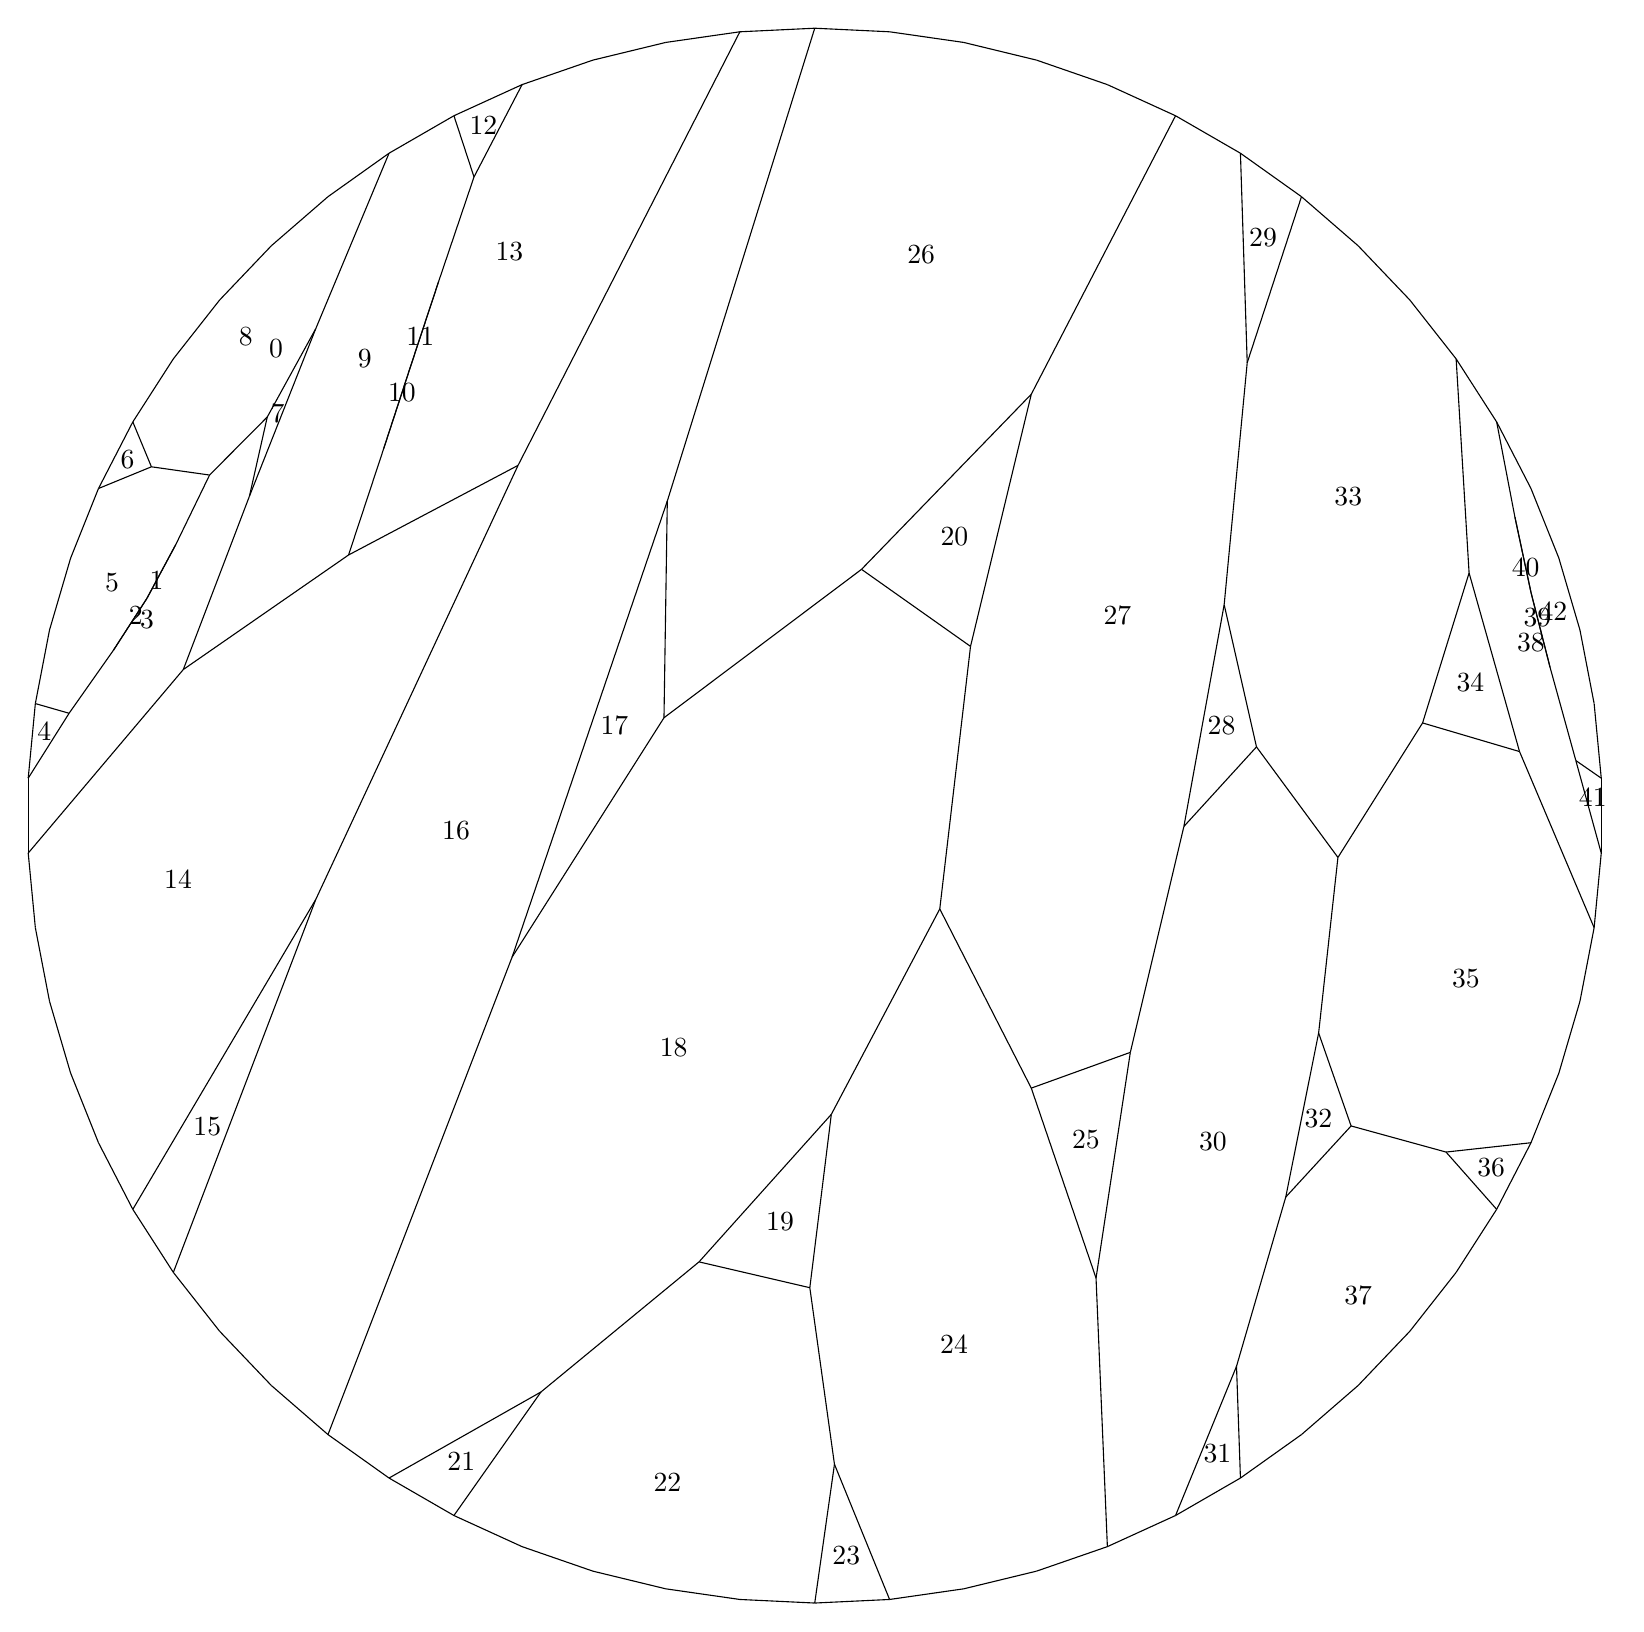
\begin{tikzpicture}[scale = 10, auto]
\coordinate (x0) at (-0.848192, 0.275787);
\coordinate (x1) at (-0.848192, 0.275787);
\coordinate (x2) at (-0.811383, 0.344377);
\coordinate (x3) at (-0.890438, 0.210336);
\coordinate (x4) at (-0.946964, 0.129992);
\coordinate (x5) at (-0.998867, 0.047582);
\coordinate (x6) at (-0.998867, -0.047582);
\coordinate (x7) at (-0.801909, 0.185524);
\coordinate (x8) at (-0.717923, 0.405637);
\coordinate (x9) at (-0.695270, 0.506283);
\coordinate (x10) at (-0.768539, 0.432537);
\coordinate (x11) at (-0.989821, 0.142315);
\coordinate (x12) at (-0.842414, 0.443009);
\coordinate (x13) at (-0.909632, 0.415415);
\coordinate (x14) at (-0.945001, 0.327068);
\coordinate (x15) at (-0.971812, 0.235759);
\coordinate (x16) at (-0.866025, 0.500000);
\coordinate (x17) at (-0.633684, 0.618459);
\coordinate (x18) at (-0.540641, 0.841254);
\coordinate (x19) at (-0.618159, 0.786053);
\coordinate (x20) at (-0.690079, 0.723734);
\coordinate (x21) at (-0.755750, 0.654861);
\coordinate (x22) at (-0.814576, 0.580057);
\coordinate (x23) at (-0.592048, 0.331009);
\coordinate (x24) at (-0.547488, 0.465891);
\coordinate (x25) at (-0.512560, 0.572744);
\coordinate (x26) at (-0.477567, 0.678540);
\coordinate (x27) at (-0.432725, 0.811127);
\coordinate (x28) at (-0.458227, 0.888835);
\coordinate (x29) at (-0.512560, 0.572744);
\coordinate (x30) at (-0.371662, 0.928368);
\coordinate (x31) at (-0.376795, 0.444815);
\coordinate (x32) at (-0.095056, 0.995472);
\coordinate (x33) at (-0.189251, 0.981929);
\coordinate (x34) at (-0.281733, 0.959493);
\coordinate (x35) at (-0.989821, -0.142315);
\coordinate (x36) at (-0.971812, -0.235759);
\coordinate (x37) at (-0.945001, -0.327068);
\coordinate (x38) at (-0.909632, -0.415415);
\coordinate (x39) at (-0.866025, -0.500000);
\coordinate (x40) at (-0.633673, -0.106447);
\coordinate (x41) at (-0.814576, -0.580057);
\coordinate (x42) at (-0.755750, -0.654861);
\coordinate (x43) at (-0.690079, -0.723734);
\coordinate (x44) at (-0.618159, -0.786053);
\coordinate (x45) at (-0.384345, -0.179661);
\coordinate (x46) at (-0.187239, 0.399502);
\coordinate (x47) at (0.000000, 1.000000);
\coordinate (x48) at (-0.191448, 0.124305);
\coordinate (x49) at (-0.540641, -0.841254);
\coordinate (x50) at (-0.347712, -0.731977);
\coordinate (x51) at (-0.146937, -0.566728);
\coordinate (x52) at (0.021058, -0.379395);
\coordinate (x53) at (0.158792, -0.118539);
\coordinate (x54) at (0.197842, 0.214930);
\coordinate (x55) at (0.059411, 0.312769);
\coordinate (x56) at (-0.006243, -0.599512);
\coordinate (x57) at (0.275020, 0.535177);
\coordinate (x58) at (-0.458227, -0.888835);
\coordinate (x59) at (-0.371662, -0.928368);
\coordinate (x60) at (-0.281733, -0.959493);
\coordinate (x61) at (-0.189251, -0.981929);
\coordinate (x62) at (-0.095056, -0.995472);
\coordinate (x63) at (-0.000000, -1.000000);
\coordinate (x64) at (0.025059, -0.823799);
\coordinate (x65) at (0.095056, -0.995472);
\coordinate (x66) at (0.189251, -0.981929);
\coordinate (x67) at (0.281733, -0.959493);
\coordinate (x68) at (0.371662, -0.928368);
\coordinate (x69) at (0.357257, -0.587304);
\coordinate (x70) at (0.275028, -0.346065);
\coordinate (x71) at (0.400807, -0.300641);
\coordinate (x72) at (0.458227, 0.888835);
\coordinate (x73) at (0.371662, 0.928368);
\coordinate (x74) at (0.281733, 0.959493);
\coordinate (x75) at (0.189251, 0.981929);
\coordinate (x76) at (0.095056, 0.995472);
\coordinate (x77) at (0.468827, -0.013734);
\coordinate (x78) at (0.519981, 0.267876);
\coordinate (x79) at (0.549236, 0.575166);
\coordinate (x80) at (0.540641, 0.841254);
\coordinate (x81) at (0.561017, 0.087293);
\coordinate (x82) at (0.618159, 0.786053);
\coordinate (x83) at (0.458227, -0.888835);
\coordinate (x84) at (0.535654, -0.699326);
\coordinate (x85) at (0.598196, -0.484402);
\coordinate (x86) at (0.639935, -0.276047);
\coordinate (x87) at (0.664466, -0.053100);
\coordinate (x88) at (0.540641, -0.841254);
\coordinate (x89) at (0.681173, -0.394111);
\coordinate (x90) at (0.771956, 0.117723);
\coordinate (x91) at (0.831022, 0.308177);
\coordinate (x92) at (0.814576, 0.580057);
\coordinate (x93) at (0.755750, 0.654861);
\coordinate (x94) at (0.690079, 0.723734);
\coordinate (x95) at (0.895079, 0.081366);
\coordinate (x96) at (0.801738, -0.427259);
\coordinate (x97) at (0.909632, -0.415415);
\coordinate (x98) at (0.945001, -0.327068);
\coordinate (x99) at (0.971812, -0.235759);
\coordinate (x100) at (0.989821, -0.142315);
\coordinate (x101) at (0.866025, -0.500000);
\coordinate (x102) at (0.618159, -0.786053);
\coordinate (x103) at (0.690079, -0.723734);
\coordinate (x104) at (0.755750, -0.654861);
\coordinate (x105) at (0.814576, -0.580057);
\coordinate (x106) at (0.998867, -0.047582);
\coordinate (x107) at (0.966576, 0.069967);
\coordinate (x108) at (0.933805, 0.188546);
\coordinate (x109) at (0.909686, 0.283219);
\coordinate (x110) at (0.889274, 0.378876);
\coordinate (x111) at (0.866025, 0.500000);
\coordinate (x112) at (0.909689, 0.283220);
\coordinate (x113) at (0.998867, 0.047582);
\coordinate (x114) at (0.989821, 0.142315);
\coordinate (x115) at (0.971812, 0.235759);
\coordinate (x116) at (0.945001, 0.327068);
\coordinate (x117) at (0.909632, 0.415415);
\draw (-0.848192, 0.275787) -- (-0.848192, 0.275787);
\draw (-0.848192, 0.275787) -- (-0.811383, 0.344377);
\draw (-0.811383, 0.344377) -- (-0.848192, 0.275787);
\draw (-0.848192, 0.275787) -- (-0.890438, 0.210336);
\draw (-0.890438, 0.210336) -- (-0.848192, 0.275787);
\draw (-0.890438, 0.210336) -- (-0.946964, 0.129992);
\draw (-0.946964, 0.129992) -- (-0.998867, 0.047582);
\draw (-0.998867, 0.047582) -- (-0.998867, -0.047582);
\draw (-0.998867, -0.047582) -- (-0.801909, 0.185524);
\draw (-0.801909, 0.185524) -- (-0.717923, 0.405637);
\draw (-0.717923, 0.405637) -- (-0.695270, 0.506283);
\draw (-0.695270, 0.506283) -- (-0.768539, 0.432537);
\draw (-0.768539, 0.432537) -- (-0.811383, 0.344377);
\draw (-0.946964, 0.129992) -- (-0.989821, 0.142315);
\draw (-0.989821, 0.142315) -- (-0.998867, 0.047582);
\draw (-0.768539, 0.432537) -- (-0.842414, 0.443009);
\draw (-0.842414, 0.443009) -- (-0.909632, 0.415415);
\draw (-0.909632, 0.415415) -- (-0.945001, 0.327068);
\draw (-0.945001, 0.327068) -- (-0.971812, 0.235759);
\draw (-0.971812, 0.235759) -- (-0.989821, 0.142315);
\draw (-0.842414, 0.443009) -- (-0.866025, 0.500000);
\draw (-0.866025, 0.500000) -- (-0.909632, 0.415415);
\draw (-0.717923, 0.405637) -- (-0.633684, 0.618459);
\draw (-0.633684, 0.618459) -- (-0.695270, 0.506283);
\draw (-0.633684, 0.618459) -- (-0.540641, 0.841254);
\draw (-0.540641, 0.841254) -- (-0.618159, 0.786053);
\draw (-0.618159, 0.786053) -- (-0.690079, 0.723734);
\draw (-0.690079, 0.723734) -- (-0.755750, 0.654861);
\draw (-0.755750, 0.654861) -- (-0.814576, 0.580057);
\draw (-0.814576, 0.580057) -- (-0.866025, 0.500000);
\draw (-0.801909, 0.185524) -- (-0.592048, 0.331009);
\draw (-0.592048, 0.331009) -- (-0.547488, 0.465891);
\draw (-0.547488, 0.465891) -- (-0.512560, 0.572744);
\draw (-0.512560, 0.572744) -- (-0.477567, 0.678540);
\draw (-0.477567, 0.678540) -- (-0.432725, 0.811127);
\draw (-0.432725, 0.811127) -- (-0.458227, 0.888835);
\draw (-0.458227, 0.888835) -- (-0.540641, 0.841254);
\draw (-0.547488, 0.465891) -- (-0.512560, 0.572744);
\draw (-0.512560, 0.572744) -- (-0.512560, 0.572744);
\draw (-0.512560, 0.572744) -- (-0.477567, 0.678540);
\draw (-0.432725, 0.811127) -- (-0.371662, 0.928368);
\draw (-0.371662, 0.928368) -- (-0.458227, 0.888835);
\draw (-0.592048, 0.331009) -- (-0.376795, 0.444815);
\draw (-0.376795, 0.444815) -- (-0.095056, 0.995472);
\draw (-0.095056, 0.995472) -- (-0.189251, 0.981929);
\draw (-0.189251, 0.981929) -- (-0.281733, 0.959493);
\draw (-0.281733, 0.959493) -- (-0.371662, 0.928368);
\draw (-0.998867, -0.047582) -- (-0.989821, -0.142315);
\draw (-0.989821, -0.142315) -- (-0.971812, -0.235759);
\draw (-0.971812, -0.235759) -- (-0.945001, -0.327068);
\draw (-0.945001, -0.327068) -- (-0.909632, -0.415415);
\draw (-0.909632, -0.415415) -- (-0.866025, -0.500000);
\draw (-0.866025, -0.500000) -- (-0.633673, -0.106447);
\draw (-0.633673, -0.106447) -- (-0.376795, 0.444815);
\draw (-0.866025, -0.500000) -- (-0.814576, -0.580057);
\draw (-0.814576, -0.580057) -- (-0.633673, -0.106447);
\draw (-0.814576, -0.580057) -- (-0.755750, -0.654861);
\draw (-0.755750, -0.654861) -- (-0.690079, -0.723734);
\draw (-0.690079, -0.723734) -- (-0.618159, -0.786053);
\draw (-0.618159, -0.786053) -- (-0.384345, -0.179661);
\draw (-0.384345, -0.179661) -- (-0.187239, 0.399502);
\draw (-0.187239, 0.399502) -- (0.000000, 1.000000);
\draw (0.000000, 1.000000) -- (-0.095056, 0.995472);
\draw (-0.384345, -0.179661) -- (-0.191448, 0.124305);
\draw (-0.191448, 0.124305) -- (-0.187239, 0.399502);
\draw (-0.618159, -0.786053) -- (-0.540641, -0.841254);
\draw (-0.540641, -0.841254) -- (-0.347712, -0.731977);
\draw (-0.347712, -0.731977) -- (-0.146937, -0.566728);
\draw (-0.146937, -0.566728) -- (0.021058, -0.379395);
\draw (0.021058, -0.379395) -- (0.158792, -0.118539);
\draw (0.158792, -0.118539) -- (0.197842, 0.214930);
\draw (0.197842, 0.214930) -- (0.059411, 0.312769);
\draw (0.059411, 0.312769) -- (-0.191448, 0.124305);
\draw (-0.146937, -0.566728) -- (-0.006243, -0.599512);
\draw (-0.006243, -0.599512) -- (0.021058, -0.379395);
\draw (0.197842, 0.214930) -- (0.275020, 0.535177);
\draw (0.275020, 0.535177) -- (0.059411, 0.312769);
\draw (-0.540641, -0.841254) -- (-0.458227, -0.888835);
\draw (-0.458227, -0.888835) -- (-0.347712, -0.731977);
\draw (-0.458227, -0.888835) -- (-0.371662, -0.928368);
\draw (-0.371662, -0.928368) -- (-0.281733, -0.959493);
\draw (-0.281733, -0.959493) -- (-0.189251, -0.981929);
\draw (-0.189251, -0.981929) -- (-0.095056, -0.995472);
\draw (-0.095056, -0.995472) -- (-0.000000, -1.000000);
\draw (-0.000000, -1.000000) -- (0.025059, -0.823799);
\draw (0.025059, -0.823799) -- (-0.006243, -0.599512);
\draw (-0.000000, -1.000000) -- (0.095056, -0.995472);
\draw (0.095056, -0.995472) -- (0.025059, -0.823799);
\draw (0.095056, -0.995472) -- (0.189251, -0.981929);
\draw (0.189251, -0.981929) -- (0.281733, -0.959493);
\draw (0.281733, -0.959493) -- (0.371662, -0.928368);
\draw (0.371662, -0.928368) -- (0.357257, -0.587304);
\draw (0.357257, -0.587304) -- (0.275028, -0.346065);
\draw (0.275028, -0.346065) -- (0.158792, -0.118539);
\draw (0.357257, -0.587304) -- (0.400807, -0.300641);
\draw (0.400807, -0.300641) -- (0.275028, -0.346065);
\draw (0.275020, 0.535177) -- (0.458227, 0.888835);
\draw (0.458227, 0.888835) -- (0.371662, 0.928368);
\draw (0.371662, 0.928368) -- (0.281733, 0.959493);
\draw (0.281733, 0.959493) -- (0.189251, 0.981929);
\draw (0.189251, 0.981929) -- (0.095056, 0.995472);
\draw (0.095056, 0.995472) -- (0.000000, 1.000000);
\draw (0.400807, -0.300641) -- (0.468827, -0.013734);
\draw (0.468827, -0.013734) -- (0.519981, 0.267876);
\draw (0.519981, 0.267876) -- (0.549236, 0.575166);
\draw (0.549236, 0.575166) -- (0.540641, 0.841254);
\draw (0.540641, 0.841254) -- (0.458227, 0.888835);
\draw (0.468827, -0.013734) -- (0.561017, 0.087293);
\draw (0.561017, 0.087293) -- (0.519981, 0.267876);
\draw (0.549236, 0.575166) -- (0.618159, 0.786053);
\draw (0.618159, 0.786053) -- (0.540641, 0.841254);
\draw (0.371662, -0.928368) -- (0.458227, -0.888835);
\draw (0.458227, -0.888835) -- (0.535654, -0.699326);
\draw (0.535654, -0.699326) -- (0.598196, -0.484402);
\draw (0.598196, -0.484402) -- (0.639935, -0.276047);
\draw (0.639935, -0.276047) -- (0.664466, -0.053100);
\draw (0.664466, -0.053100) -- (0.561017, 0.087293);
\draw (0.458227, -0.888835) -- (0.540641, -0.841254);
\draw (0.540641, -0.841254) -- (0.535654, -0.699326);
\draw (0.598196, -0.484402) -- (0.681173, -0.394111);
\draw (0.681173, -0.394111) -- (0.639935, -0.276047);
\draw (0.664466, -0.053100) -- (0.771956, 0.117723);
\draw (0.771956, 0.117723) -- (0.831022, 0.308177);
\draw (0.831022, 0.308177) -- (0.814576, 0.580057);
\draw (0.814576, 0.580057) -- (0.755750, 0.654861);
\draw (0.755750, 0.654861) -- (0.690079, 0.723734);
\draw (0.690079, 0.723734) -- (0.618159, 0.786053);
\draw (0.771956, 0.117723) -- (0.895079, 0.081366);
\draw (0.895079, 0.081366) -- (0.831022, 0.308177);
\draw (0.681173, -0.394111) -- (0.801738, -0.427259);
\draw (0.801738, -0.427259) -- (0.909632, -0.415415);
\draw (0.909632, -0.415415) -- (0.945001, -0.327068);
\draw (0.945001, -0.327068) -- (0.971812, -0.235759);
\draw (0.971812, -0.235759) -- (0.989821, -0.142315);
\draw (0.989821, -0.142315) -- (0.895079, 0.081366);
\draw (0.801738, -0.427259) -- (0.866025, -0.500000);
\draw (0.866025, -0.500000) -- (0.909632, -0.415415);
\draw (0.540641, -0.841254) -- (0.618159, -0.786053);
\draw (0.618159, -0.786053) -- (0.690079, -0.723734);
\draw (0.690079, -0.723734) -- (0.755750, -0.654861);
\draw (0.755750, -0.654861) -- (0.814576, -0.580057);
\draw (0.814576, -0.580057) -- (0.866025, -0.500000);
\draw (0.989821, -0.142315) -- (0.998867, -0.047582);
\draw (0.998867, -0.047582) -- (0.966576, 0.069967);
\draw (0.966576, 0.069967) -- (0.933805, 0.188546);
\draw (0.933805, 0.188546) -- (0.909686, 0.283219);
\draw (0.909686, 0.283219) -- (0.889274, 0.378876);
\draw (0.889274, 0.378876) -- (0.866025, 0.500000);
\draw (0.866025, 0.500000) -- (0.814576, 0.580057);
\draw (0.933805, 0.188546) -- (0.909689, 0.283220);
\draw (0.909689, 0.283220) -- (0.909686, 0.283219);
\draw (0.909689, 0.283220) -- (0.889274, 0.378876);
\draw (0.998867, -0.047582) -- (0.998867, 0.047582);
\draw (0.998867, 0.047582) -- (0.966576, 0.069967);
\draw (0.998867, 0.047582) -- (0.989821, 0.142315);
\draw (0.989821, 0.142315) -- (0.971812, 0.235759);
\draw (0.971812, 0.235759) -- (0.945001, 0.327068);
\draw (0.945001, 0.327068) -- (0.909632, 0.415415);
\draw (0.909632, 0.415415) -- (0.866025, 0.500000);
\node at (-0.684262, 0.592917) {0};
\node at (-0.835922, 0.298650) {1};
\node at (-0.862274, 0.253970) {2};
\node at (-0.847835, 0.249047) {3};
\node at (-0.978551, 0.106629) {4};
\node at (-0.892420, 0.295659) {5};
\node at (-0.872690, 0.452808) {6};
\node at (-0.682292, 0.510126) {7};
\node at (-0.722514, 0.608625) {8};
\node at (-0.571477, 0.579902) {9};
\node at (-0.524202, 0.537126) {10};
\node at (-0.500895, 0.608009) {11};
\node at (-0.420871, 0.876110) {12};
\node at (-0.387688, 0.716939) {13};
\node at (-0.808558, -0.081324) {14};
\node at (-0.771425, -0.395501) {15};
\node at (-0.455567, -0.019102) {16};
\node at (-0.254344, 0.114715) {17};
\node at (-0.179214, -0.295160) {18};
\node at (-0.044041, -0.515212) {19};
\node at (0.177424, 0.354292) {20};
\node at (-0.448860, -0.820689) {21};
\node at (-0.187176, -0.847611) {22};
\node at (0.040038, -0.939757) {23};
\node at (0.176865, -0.671988) {24};
\node at (0.344364, -0.411337) {25};
\node at (0.135167, 0.712585) {26};
\node at (0.384440, 0.254426) {27};
\node at (0.516609, 0.113811) {28};
\node at (0.569345, 0.734158) {29};
\node at (0.505605, -0.414446) {30};
\node at (0.511507, -0.809805) {31};
\node at (0.639768, -0.384853) {32};
\node at (0.677624, 0.404784) {33};
\node at (0.832686, 0.169088) {34};
\node at (0.827061, -0.207198) {35};
\node at (0.859132, -0.447558) {36};
\node at (0.690199, -0.609106) {37};
\node at (0.909473, 0.220031) {38};
\node at (0.917727, 0.251661) {39};
\node at (0.902883, 0.315105) {40};
\node at (0.988103, 0.023322) {41};
\node at (0.938050, 0.258875) {42};
\end{tikzpicture}
\caption{Graph}

\end{figure}
\end{document}

        % \end{scope}
        \\
      };
      % \begin{scope}[scale=3]
      %   \documentclass[a4paper]{article}
\usepackage[left=0.5cm, right=0.5cm, top=1cm, bottom=1cm]{geometry}
\usepackage{tikz}
\begin{document}
\begin{figure}[h!]
\centering
\begin{tikzpicture}[scale = 10, auto]
\coordinate (x0) at (0.166104, 0.013310);
\coordinate (x1) at (0.138873, -0.202200);
\coordinate (x2) at (0.386369, -0.560024);
\coordinate (x3) at (0.748511, -0.663123);
\coordinate (x4) at (0.970942, -0.239316);
\coordinate (x5) at (0.794923, 0.001403);
\coordinate (x6) at (0.480588, 0.007178);
\coordinate (x7) at (-0.131665, 0.121253);
\coordinate (x8) at (0.354605, -0.935016);
\coordinate (x9) at (0.970942, 0.239316);
\coordinate (x10) at (0.748511, 0.663123);
\coordinate (x11) at (0.354605, 0.935016);
\coordinate (x12) at (-0.120537, 0.992709);
\coordinate (x13) at (-0.568065, 0.822984);
\coordinate (x14) at (-0.484996, 0.430986);
\coordinate (x15) at (-0.885456, 0.464723);
\coordinate (x16) at (-1.000000, 0.000000);
\coordinate (x17) at (-0.885456, -0.464723);
\coordinate (x18) at (-0.568065, -0.822984);
\coordinate (x19) at (-0.120537, -0.992709);
\draw (0.166104, 0.013310) -- (0.138873, -0.202200);
\draw (0.138873, -0.202200) -- (0.386369, -0.560024);
\draw (0.386369, -0.560024) -- (0.748511, -0.663123);
\draw (0.748511, -0.663123) -- (0.970942, -0.239316);
\draw (0.970942, -0.239316) -- (0.794923, 0.001403);
\draw (0.794923, 0.001403) -- (0.480588, 0.007178);
\draw (0.480588, 0.007178) -- (0.166104, 0.013310);
\draw (0.166104, 0.013310) -- (-0.131665, 0.121253);
\draw (-0.131665, 0.121253) -- (0.138873, -0.202200);
\draw (0.386369, -0.560024) -- (0.354605, -0.935016);
\draw (0.354605, -0.935016) -- (0.748511, -0.663123);
\draw (0.970942, -0.239316) -- (0.970942, 0.239316);
\draw (0.970942, 0.239316) -- (0.794923, 0.001403);
\draw (0.970942, 0.239316) -- (0.748511, 0.663123);
\draw (0.748511, 0.663123) -- (0.354605, 0.935016);
\draw (0.354605, 0.935016) -- (-0.120537, 0.992709);
\draw (-0.120537, 0.992709) -- (-0.568065, 0.822984);
\draw (-0.568065, 0.822984) -- (-0.484996, 0.430986);
\draw (-0.484996, 0.430986) -- (-0.131665, 0.121253);
\draw (-0.568065, 0.822984) -- (-0.885456, 0.464723);
\draw (-0.885456, 0.464723) -- (-0.484996, 0.430986);
\draw (-0.885456, 0.464723) -- (-1.000000, 0.000000);
\draw (-1.000000, 0.000000) -- (-0.885456, -0.464723);
\draw (-0.885456, -0.464723) -- (-0.568065, -0.822984);
\draw (-0.568065, -0.822984) -- (-0.120537, -0.992709);
\draw (-0.120537, -0.992709) -- (0.354605, -0.935016);
\node at (-0.000000, 0.000000) {0};
\node at (0.526616, -0.234682) {1};
\node at (0.057771, -0.022546) {2};
\node at (0.496495, -0.719388) {3};
\node at (0.912269, 0.000468) {4};
\node at (0.221041, 0.422728) {5};
\node at (-0.646172, 0.572898) {6};
\node at (-0.319633, -0.296069) {7};
\end{tikzpicture}
\caption{Graph}

\end{figure}
\end{document}

      % \end{scope}


    \end{tikzfigure}
  \end{proof}
\end{theorem}